\section[Union-Find]{Rappresentazione di partizioni (UNION-FIND)}
Dato un insieme $\mathcal{A}$, una partizione è una famiglia di sottoinsiemi $\mathcal{A}_{1...k}$ tali che 
\begin{itemize}
    \item $\mathcal{A}_{i} \neq \emptyset$
    \item  $\mathcal{A}_{i} \cap \mathcal{A}_{j} = \emptyset$
    \item $\mathcal{A}_{1} \cup ... \cup \mathcal{A}_{k} = \mathcal{A}$
\end{itemize}

Vogliamo rappresentare una collezione di insiemi disgiunti mediante le operazioni:
\begin{itemize}
    \item \texttt{UNION(A, B)} unisce gli insiemi $A$ e $B$ in un unico insieme $A$
    \item \texttt{FIND(X)} restituisce il nome dell'insieme che contiene l'elemento $x$
    \item \texttt{MAKESET(X)} crea un nuovo insieme $\lbrace x \rbrace$ di nome $X$ ($x$ nuovo elemento)
\end{itemize}

\noindent Ogni insieme è rappresentato da un albero con radice con puntatori verso l'alto, dove i nodi sono 
gli elementi dell'insieme e la radice è il nome dell'insieme. Una partizione è quindi una foresta di alberi.
In base a come impostiamo il nostro sistema di partizioni possiamo velocizzare le \texttt{UNION} 
oppure le \texttt{FIND}.

\subsection{Operazioni QUICKFIND}
\begin{wrapfigure}{r}{7cm}
    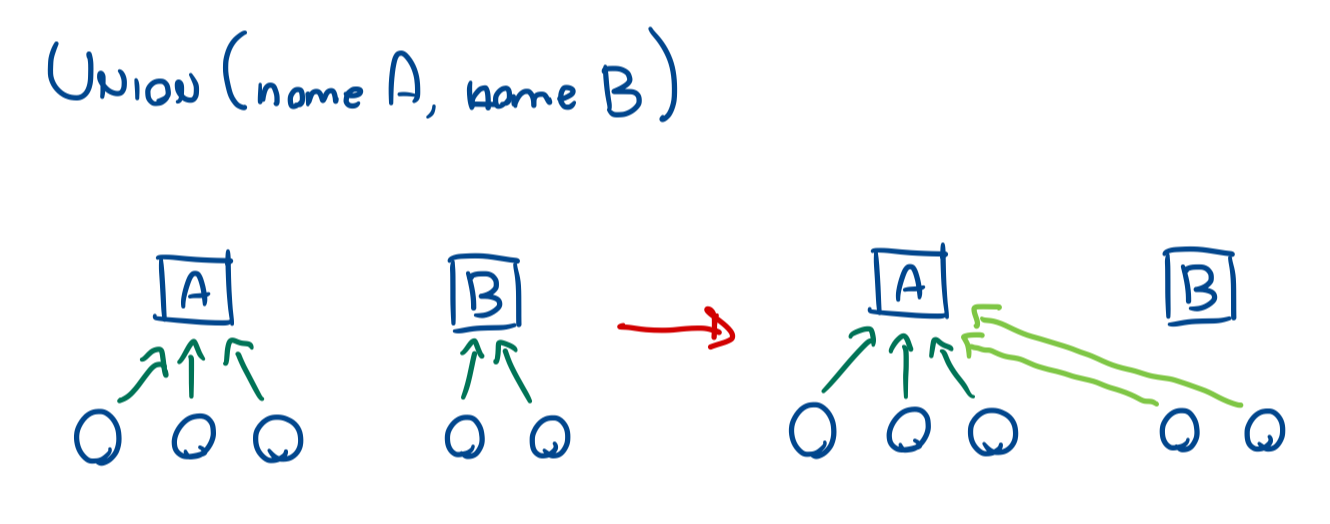
\includegraphics[scale = 0.3]{quickfind-union.png}
\end{wrapfigure}
Considero alberi di altezza 1 dove gli elementi dell'insieme sono le foglie
e il nome dell'insieme è dato dalla radice.
Quando $n(A) > n(B)$ conviene spostare gli elementi di $B$ sotto ad $A$ e cambiare
nome alla radice. Per ottimizzare, durante \texttt{Makeset} memorizzo nella radice
il numero di elementi dell'insieme. Quando poi faccio union sommo il numero di elementi.
Lo spazio è lineare rispetto a $n$ quindi è $O(n)$.\\
Effettuando una sequenza di $n$ \texttt{makeset} e $O(n)$ \texttt{union} e \texttt{find}
ottengo un costo ammortizzato $O(\log n)$
\clearpage

\subsection{Operazioni QUICKUNION}
Gli alberi non sono più vincolati ad avere altezza 1 e la radice contiene il nome dell'insieme.
Al contrario delle operazioni QUICKFIND queste favoriscono in termini di 
complessità l'implementazione della funzione \texttt{UNION}.
\begin{figure}[h]
    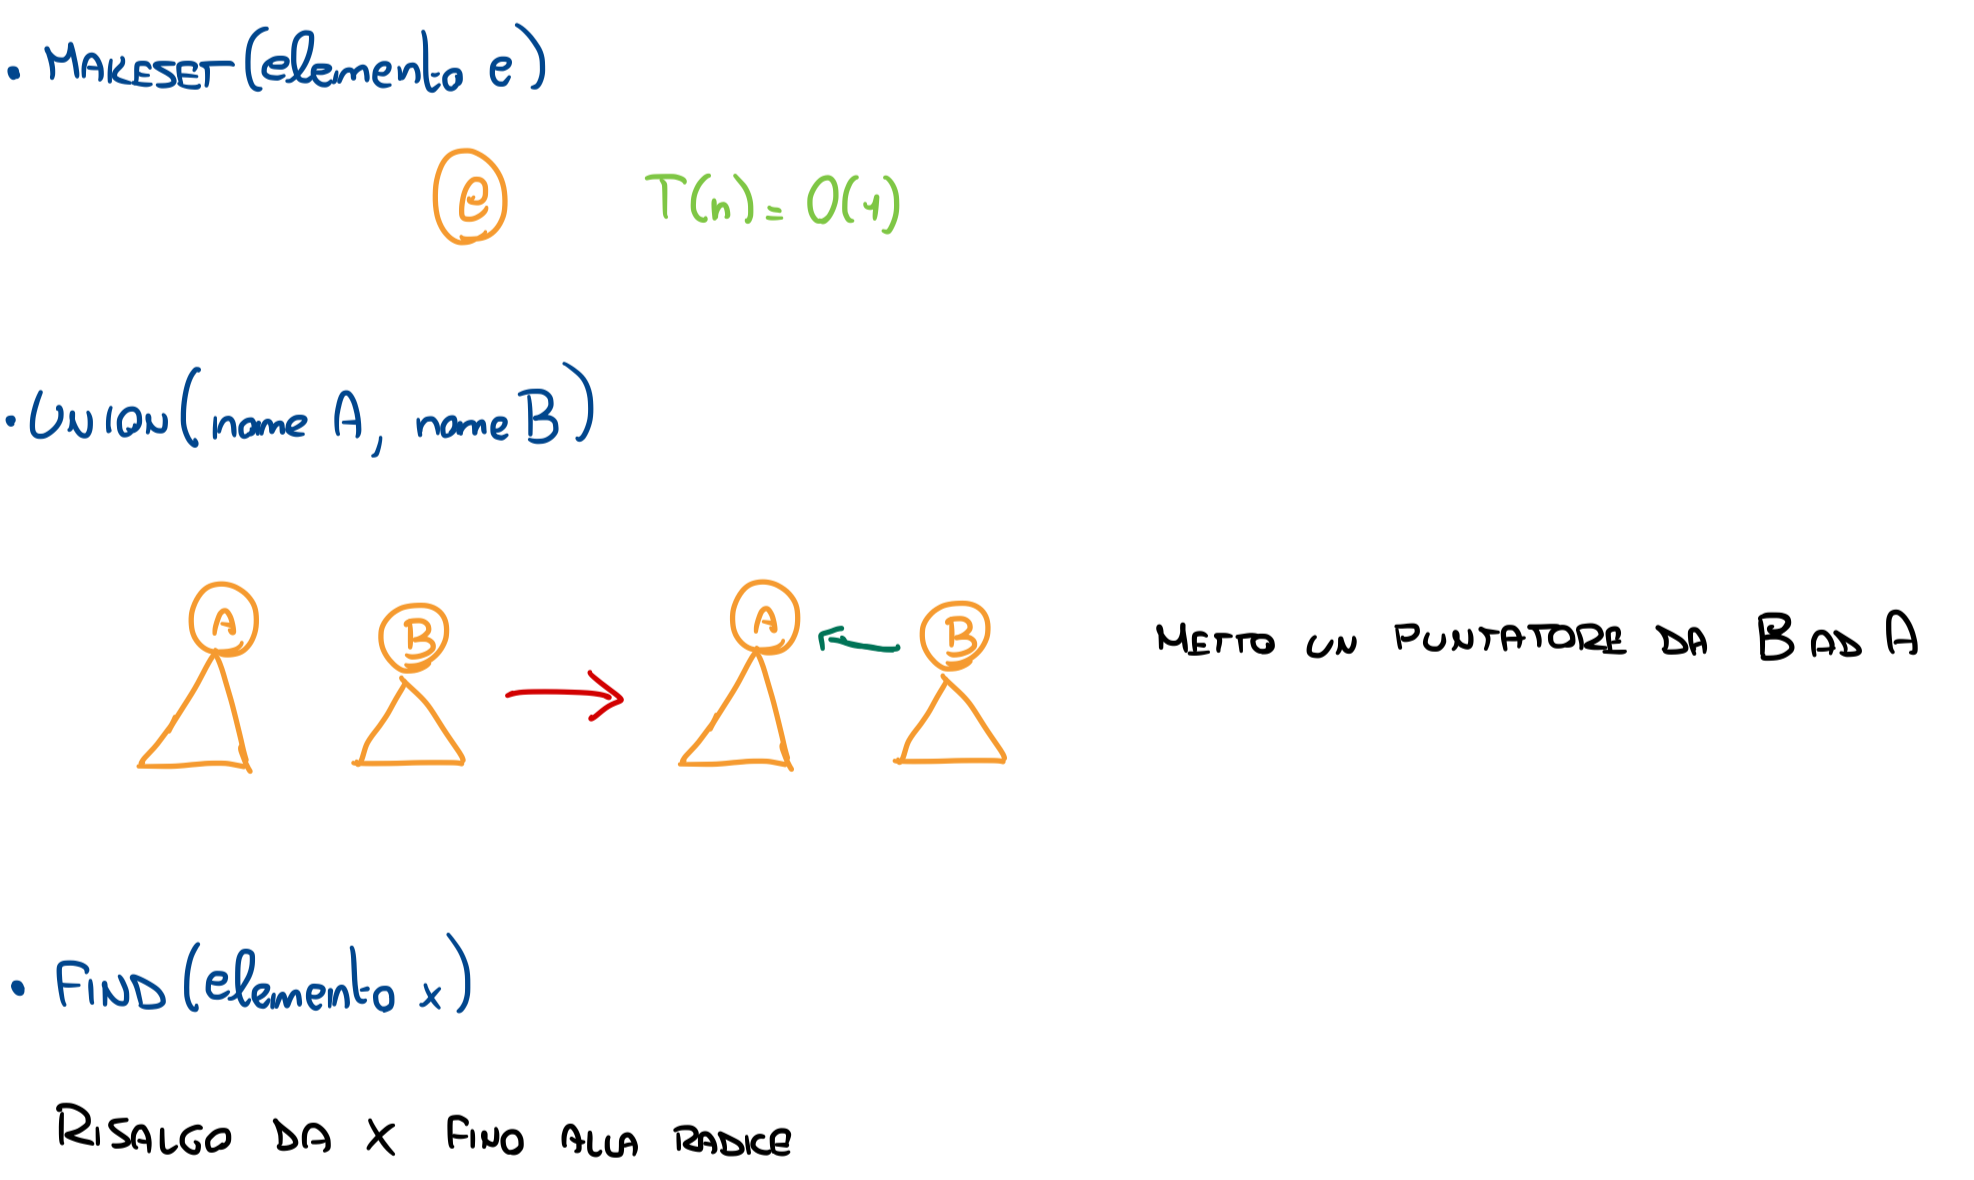
\includegraphics[width=\textwidth]{quickunion.png}
\end{figure}

\subsection{Algoritmo QUICKFIND bilanciato}
L'utilizzo della rappresentazione QUICKFIND penalizza l'operazione di \texttt{UNION}.
È possibile eseguire alcuni miglioramenti al fine di migliorare la complessità di tale operazione.\\
Gli accorgimenti che si possono introdurre sono:
\begin{enumerate}
    \item Memorizzare all'interno di ogni albero la cardinalità dell'insieme, ovvero
    il numero di foglie dell'albero.
    \item Nella realizzazione dell'operazione \texttt{UNION(A, B)}:
    \begin{enumerate}
        \item Spostare le foglie dell'albero rappresentante l'insieme di cardinalità 
        minore verso l'albero rappresentante l'insieme di cardinalità maggiore;
        \item Memorizzare l'etichetta da associare al nuovo insieme all'interno della radice
        dell'albero rappresentante l'insieme unione.

    \end{enumerate}
\end{enumerate}

Il tempo utilizzato dalla \texttt{UNION} di questo algoritmo bilanciato è logaritmico
rispetto al numero di \texttt{MAKESET} effettuate, ovvero rispetto al numero di 
elementi contenuti nella foresta di alberi.

\subsection{Algoritmo QUICKUNION bilanciato}
In maniera speculare rispetto al QUICKFIND bilanciato, è possibile adottare alcuni 
accorgimenti per controllare l'altezza dell'albero rappresentante l'insieme e quindi
migliorare l'esecuzione di \texttt{FIND}.
\subsubsection*{Union by rank}
È una variante della rappresentazione QUICKUNION che, al fine di evitare che l'altezza dell'albero cresca senza alcun controllo,
adotta i seguenti accorgimenti:
\begin{enumerate}
    \item Memorizza all'interno di ogni radice l'altezza dell'albero
    \item Nella realizzazione dell'operazione di \texttt{UNION(A, B)}:
    \begin{enumerate}
        \item La radice dell'albero avente altezza maggiore diventa padre della radice
        dell'albero avente altezza minore
        \item memorizza l'etichetta da associare al nuovo insieme all'interno del nodo 
        diventato radice dell'albero unione
    \end{enumerate}
\end{enumerate}

\textbf{Lemma:}
\begin{center}
    Ogni albero QUICKUNION bilanciato in altezza con radice $x$ contiene almeno
    $2^{rank(x)}$ nodi.
\end{center}

\subsection{Compressione di cammino} 
Sempre nell'ambito della rappresentazione QUICKUNION è possibile introdurre ulteriori accorgimenti
volti a migliorare la complessità dell'operazione di \texttt{FIND}.
La compressione di cammino si serve dell'algoritmo di \texttt{FIND} facendo leva 
sul movimento che esso esegue nella ricerca dell'etichetta posta alla radice.
L'idea della compressione di cammino è quella di assegnare un ulteriore compito al \texttt{FIND}, 
ovvero quello di ristrutturare l'albero ponendo il padre di ogni nodo incontrato uguale
alla radice dell'albero. Eseguiamo in tal modo una compressione dell'altezza dell'albero 
lungo tutto il cammino che dal nodo contenente l'elemento da trovare termina nella radice.

\subsection{Riepilogo costi operazioni}
\begin{tabular}{|l|c|c|c|}
    \hline
    \space & \textbf{MAKESET} & \textbf{UNION} & \textbf{FIND}\\
    \hline
    \textbf{QUICKFIND} & $O(1)$ & $O(n)$ & $O(1)$\\
    \hline
    \textbf{QUICKFIND bilanciato} & $O(1)$ & $O(\log n)$ & $O(1)$\\
    \hline
    \textbf{QUICKUNION} & $O(1)$ & $O(1)$ & $O(n)$\\
    \hline
    \textbf{QUICKUNION bilanciato} & $O(1)$ & $O(1)$ & $O(\log n)$\\
    \hline
\end{tabular}
\clearpage

